% Options for packages loaded elsewhere
\PassOptionsToPackage{unicode}{hyperref}
\PassOptionsToPackage{hyphens}{url}
%
\documentclass[
]{book}
\usepackage{amsmath,amssymb}
\usepackage{lmodern}
\usepackage{iftex}
\ifPDFTeX
  \usepackage[T1]{fontenc}
  \usepackage[utf8]{inputenc}
  \usepackage{textcomp} % provide euro and other symbols
\else % if luatex or xetex
  \usepackage{unicode-math}
  \defaultfontfeatures{Scale=MatchLowercase}
  \defaultfontfeatures[\rmfamily]{Ligatures=TeX,Scale=1}
\fi
% Use upquote if available, for straight quotes in verbatim environments
\IfFileExists{upquote.sty}{\usepackage{upquote}}{}
\IfFileExists{microtype.sty}{% use microtype if available
  \usepackage[]{microtype}
  \UseMicrotypeSet[protrusion]{basicmath} % disable protrusion for tt fonts
}{}
\makeatletter
\@ifundefined{KOMAClassName}{% if non-KOMA class
  \IfFileExists{parskip.sty}{%
    \usepackage{parskip}
  }{% else
    \setlength{\parindent}{0pt}
    \setlength{\parskip}{6pt plus 2pt minus 1pt}}
}{% if KOMA class
  \KOMAoptions{parskip=half}}
\makeatother
\usepackage{xcolor}
\usepackage{color}
\usepackage{fancyvrb}
\newcommand{\VerbBar}{|}
\newcommand{\VERB}{\Verb[commandchars=\\\{\}]}
\DefineVerbatimEnvironment{Highlighting}{Verbatim}{commandchars=\\\{\}}
% Add ',fontsize=\small' for more characters per line
\usepackage{framed}
\definecolor{shadecolor}{RGB}{248,248,248}
\newenvironment{Shaded}{\begin{snugshade}}{\end{snugshade}}
\newcommand{\AlertTok}[1]{\textcolor[rgb]{0.94,0.16,0.16}{#1}}
\newcommand{\AnnotationTok}[1]{\textcolor[rgb]{0.56,0.35,0.01}{\textbf{\textit{#1}}}}
\newcommand{\AttributeTok}[1]{\textcolor[rgb]{0.77,0.63,0.00}{#1}}
\newcommand{\BaseNTok}[1]{\textcolor[rgb]{0.00,0.00,0.81}{#1}}
\newcommand{\BuiltInTok}[1]{#1}
\newcommand{\CharTok}[1]{\textcolor[rgb]{0.31,0.60,0.02}{#1}}
\newcommand{\CommentTok}[1]{\textcolor[rgb]{0.56,0.35,0.01}{\textit{#1}}}
\newcommand{\CommentVarTok}[1]{\textcolor[rgb]{0.56,0.35,0.01}{\textbf{\textit{#1}}}}
\newcommand{\ConstantTok}[1]{\textcolor[rgb]{0.00,0.00,0.00}{#1}}
\newcommand{\ControlFlowTok}[1]{\textcolor[rgb]{0.13,0.29,0.53}{\textbf{#1}}}
\newcommand{\DataTypeTok}[1]{\textcolor[rgb]{0.13,0.29,0.53}{#1}}
\newcommand{\DecValTok}[1]{\textcolor[rgb]{0.00,0.00,0.81}{#1}}
\newcommand{\DocumentationTok}[1]{\textcolor[rgb]{0.56,0.35,0.01}{\textbf{\textit{#1}}}}
\newcommand{\ErrorTok}[1]{\textcolor[rgb]{0.64,0.00,0.00}{\textbf{#1}}}
\newcommand{\ExtensionTok}[1]{#1}
\newcommand{\FloatTok}[1]{\textcolor[rgb]{0.00,0.00,0.81}{#1}}
\newcommand{\FunctionTok}[1]{\textcolor[rgb]{0.00,0.00,0.00}{#1}}
\newcommand{\ImportTok}[1]{#1}
\newcommand{\InformationTok}[1]{\textcolor[rgb]{0.56,0.35,0.01}{\textbf{\textit{#1}}}}
\newcommand{\KeywordTok}[1]{\textcolor[rgb]{0.13,0.29,0.53}{\textbf{#1}}}
\newcommand{\NormalTok}[1]{#1}
\newcommand{\OperatorTok}[1]{\textcolor[rgb]{0.81,0.36,0.00}{\textbf{#1}}}
\newcommand{\OtherTok}[1]{\textcolor[rgb]{0.56,0.35,0.01}{#1}}
\newcommand{\PreprocessorTok}[1]{\textcolor[rgb]{0.56,0.35,0.01}{\textit{#1}}}
\newcommand{\RegionMarkerTok}[1]{#1}
\newcommand{\SpecialCharTok}[1]{\textcolor[rgb]{0.00,0.00,0.00}{#1}}
\newcommand{\SpecialStringTok}[1]{\textcolor[rgb]{0.31,0.60,0.02}{#1}}
\newcommand{\StringTok}[1]{\textcolor[rgb]{0.31,0.60,0.02}{#1}}
\newcommand{\VariableTok}[1]{\textcolor[rgb]{0.00,0.00,0.00}{#1}}
\newcommand{\VerbatimStringTok}[1]{\textcolor[rgb]{0.31,0.60,0.02}{#1}}
\newcommand{\WarningTok}[1]{\textcolor[rgb]{0.56,0.35,0.01}{\textbf{\textit{#1}}}}
\usepackage{longtable,booktabs,array}
\usepackage{calc} % for calculating minipage widths
% Correct order of tables after \paragraph or \subparagraph
\usepackage{etoolbox}
\makeatletter
\patchcmd\longtable{\par}{\if@noskipsec\mbox{}\fi\par}{}{}
\makeatother
% Allow footnotes in longtable head/foot
\IfFileExists{footnotehyper.sty}{\usepackage{footnotehyper}}{\usepackage{footnote}}
\makesavenoteenv{longtable}
\usepackage{graphicx}
\makeatletter
\def\maxwidth{\ifdim\Gin@nat@width>\linewidth\linewidth\else\Gin@nat@width\fi}
\def\maxheight{\ifdim\Gin@nat@height>\textheight\textheight\else\Gin@nat@height\fi}
\makeatother
% Scale images if necessary, so that they will not overflow the page
% margins by default, and it is still possible to overwrite the defaults
% using explicit options in \includegraphics[width, height, ...]{}
\setkeys{Gin}{width=\maxwidth,height=\maxheight,keepaspectratio}
% Set default figure placement to htbp
\makeatletter
\def\fps@figure{htbp}
\makeatother
\setlength{\emergencystretch}{3em} % prevent overfull lines
\providecommand{\tightlist}{%
  \setlength{\itemsep}{0pt}\setlength{\parskip}{0pt}}
\setcounter{secnumdepth}{5}
\usepackage{booktabs}
\ifLuaTeX
  \usepackage{selnolig}  % disable illegal ligatures
\fi
\usepackage[]{natbib}
\bibliographystyle{plainnat}
\IfFileExists{bookmark.sty}{\usepackage{bookmark}}{\usepackage{hyperref}}
\IfFileExists{xurl.sty}{\usepackage{xurl}}{} % add URL line breaks if available
\urlstyle{same} % disable monospaced font for URLs
\hypersetup{
  pdftitle={Exploring Simulations},
  pdfauthor={Gaston Sanchez},
  hidelinks,
  pdfcreator={LaTeX via pandoc}}

\title{Exploring Simulations}
\usepackage{etoolbox}
\makeatletter
\providecommand{\subtitle}[1]{% add subtitle to \maketitle
  \apptocmd{\@title}{\par {\large #1 \par}}{}{}
}
\makeatother
\subtitle{Simulating Games of Chance in R}
\author{Gaston Sanchez}
\date{}

\begin{document}
\maketitle

{
\setcounter{tocdepth}{1}
\tableofcontents
}
\hypertarget{about}{%
\chapter*{About}\label{about}}
\addcontentsline{toc}{chapter}{About}

\begin{center}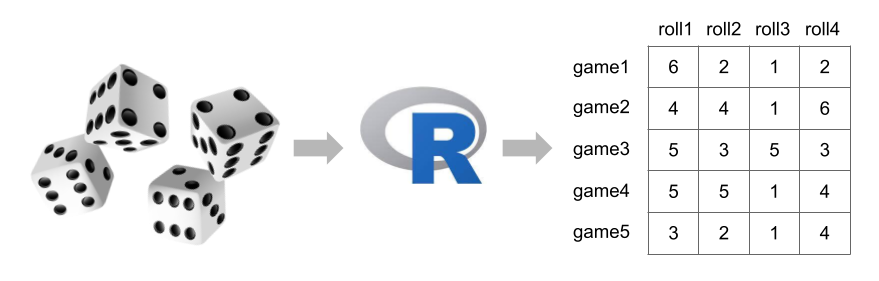
\includegraphics[width=0.9\linewidth]{images/demere-cover} \end{center}

This manuscript describes a couple of examples for implementing simulations
of games of chance.

\hypertarget{introduction}{%
\chapter{Introduction}\label{introduction}}

We are going to use a classic example in the history of probability: the
problem posed by French gambler
\href{https://en.wikipedia.org/wiki/Antoine_Gombaud}{Antoine Gombaud} (1607-1684),
better known by his \emph{nome de plume} ``Chevalier De Méré''. By the way, he was not
a nobleman, but just an amateur mathematician. Most important, for the history
of mathematics and probability, he was an avid gambler.

\begin{figure}

{\centering 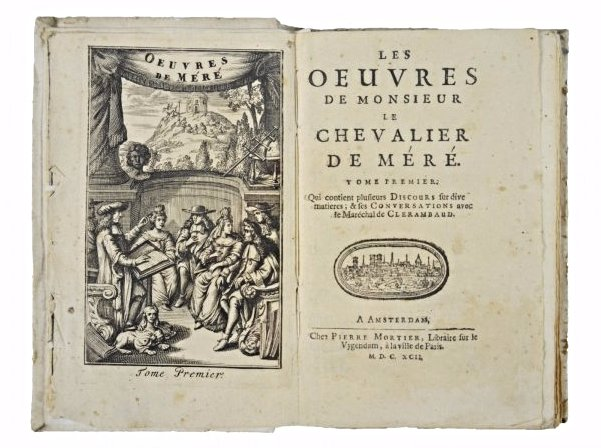
\includegraphics[width=0.6\linewidth]{images/les-ouvres-de-chevalier-demere} 

}

\caption{Old manuscript with Antoine Gombaud's texts}\label{fig:unnamed-chunk-2}
\end{figure}

Specifically, let's focus on one type of gambling scenario which we will
refer to as ``Game-A''

\hypertarget{description-of-game-a}{%
\section{Description of Game-A}\label{description-of-game-a}}

This is a fairly simple game of dice in which you roll a die four times, and
you win if you get at least one six.

\begin{figure}

{\centering 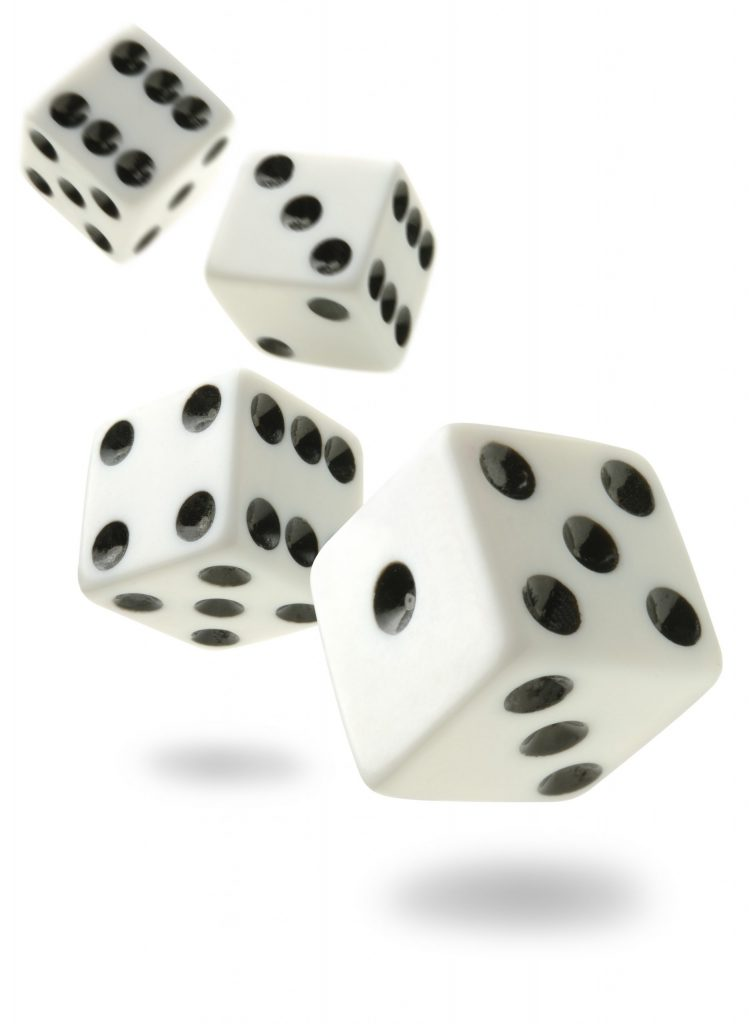
\includegraphics[width=0.3\linewidth]{images/rolling-four-dice} 

}

\caption{Rolling 4 dice in Game version A}\label{fig:unnamed-chunk-3}
\end{figure}

Think about what could happen when rolling one die four times. For instance,
some possible outcomes may be:

\begin{itemize}
\item
  \texttt{1,\ 3,\ 5,\ 2} (you lose)
\item
  \texttt{2,\ 4,\ 6,\ 5} (you win)
\item
  \texttt{5,\ 6,\ 3,\ 6} (you win)
\item
  \texttt{4,\ 2,\ 1,\ 3} (you lose)
\item
  \texttt{1,\ 3,\ 5,\ 2} (you win)
\end{itemize}

This is how De Méré was reasoning about Game-A:

\begin{itemize}
\item
  the chance of getting a six in one roll of a die is 1/6 (this is correct)
\item
  in four rolls of a die, the chance of getting one six would be
  \(4 \times 1/6 = 4/6 = 2/3\) (this is incorrect)
\end{itemize}

Based on this (incorrect) reasoning, he assumed that the odds were definitely
in his favor. Interestingly, despite De Méré's faulty reasoning about the
probability of getting one six in four rolls, he was able to make money by
playing this game.

Why was he able to make money? Let's find out the probability of winning in
this type of game.

\hypertarget{probability-of-winning-game-a}{%
\section{Probability of winning Game-A}\label{probability-of-winning-game-a}}

Finding the probability of winning Game-A translates into finding the probability
of getting at least one six in four rolls of a (fair) die:

\[
Prob(\text{winning Game-A}) = Prob(\text{getting at least one 6 in four rolls})
\]

This probability can easily be calculated with the
\emph{complementary probability rule} which states that:

\begin{quote}
the probability of one event is equal to 1 minus the probability of
its complement event.
\end{quote}

Or in symbols:

\[
Prob(\text{E}) = 1 - Prob(\text{Not E})
\]

and equivalently:

\[
Prob(\text{Not E}) = 1 - Prob(\text{E})
\]

where:

\begin{itemize}
\tightlist
\item
  \(\text{E}\) and \(\text{Not E}\) are complement events (i.e.~they cannot
  occur simultaneously)
\end{itemize}

A classic example of this type of complement events is ``E = getting heads when
flipping a coin'' and ``Not E = getting tails when flipping a coin''.

\[
Prob(\text{getting heads}) = 1 - Prob(\text{getting tails}) \\
\text{and} \\
Prob(\text{getting tails}) = 1 - Prob(\text{getting heads})
\]

So, if we consider event ``E = getting at least one six in four rolls'', then its
complement event is ``Not E = getting no six in four rolls''

\hypertarget{no-six-in-four-rolls}{%
\subsection{No six in four rolls}\label{no-six-in-four-rolls}}

The probability of getting no six in four rolls involves not getting a six
in the first roll, \emph{AND} not getting a six in the second roll, \emph{AND} not
getting a six in the third roll, \emph{AND} not getting a six in the fourth roll.
Because each roll is independent from the others, we can express this
probability as the product of the probability in each roll:

\[
Prob(\text{no 6 in 4 rolls}) = Prob(\text{no 6 in 1st roll}) \times \dots \times Prob(\text{no 6 in 4th roll})
\]

In any single roll, the probability of getting no six is:

\[
Prob(\text{no six in one roll}) = \frac{5}{6}
\]

Therefore:

\begin{align*}
Prob(\text{no six in 4 rolls}) &= Prob(\text{no 6 in 1st roll}) \times \dots \times Prob(\text{no 6 in 4th roll}) \\
&= \frac{5}{6} \times \frac{5}{6} \times \frac{5}{6} \times \frac{5}{6} \\
&= \left( \frac{5}{6} \right)^4 \\
&= \frac{625}{1296} = 0.482253
\end{align*}

Consequently, the probability of winning Game-A is:

\begin{align*}
Prob(\text{at least one six in 4 rolls}) &= 1 - Prob(\text{no six in 4 rolls}) \\
&= 1 - \left( \frac{5}{6} \right)^4 \\
&= 0.517747
\end{align*}

Note that this probability of 0.517747 is not that different from 0.5 (just
slightly greater). But the difference is enough so that if you gamble in this
game, you should expect to have a positive gain \ldots{} \textbf{in the long run}.

\hypertarget{coding-game-a}{%
\chapter{Coding Game-A}\label{coding-game-a}}

In the preceding chapter we described Game-A, and we were able to derive the
probability of winning this game:

\begin{align*}
Prob(\text{at least one six in 4 rolls}) &= 1 - Prob(\text{no six in 4 rolls}) \\
&= 1 - \left( \frac{5}{6} \right)^4 \\
&= 0.517747
\end{align*}

In this example, we are able to find the exact probability associated to the
event of ``winning Game-A''. However, not all probability problems have an
analytical solution. When this is the case, we often rely on computers to
implement simulations that allow us to find an approximate solution, and
have a better understanding of the long-term systematic patterns that arise
in random processes.

To go ahead with our exploration of simulations, let us pretend that the
probability of winning Game-A had no analytical solution. Instead, let's see
how to use R for running various simulations to get an idea of the probabilities
involved behind Game-A.

\hypertarget{rolling-one-die}{%
\section{Rolling one die}\label{rolling-one-die}}

Because Game-A involves rolling a die four times, the first step is to
create---in a computational sense---an object die, and learn how to roll it.

Perhaps the most straightforward way to create a \texttt{die} object is with a numeric
vector. One option for this is with a numeric sequence as follows:

\begin{Shaded}
\begin{Highlighting}[]
\NormalTok{die }\OtherTok{=} \DecValTok{1}\SpecialCharTok{:}\DecValTok{6}

\NormalTok{die}
\end{Highlighting}
\end{Shaded}

\begin{verbatim}
## [1] 1 2 3 4 5 6
\end{verbatim}

Once we have an object \texttt{die}, how do we roll it? Rolling a die, computationally
speaking, implies getting a sample of size 1 from the elements in vector \texttt{die}.
To do this in R, we can use the function \texttt{sample()}. This function takes an
input vector and draws a random sample---of a given size---from the vector's
elements.

\begin{Shaded}
\begin{Highlighting}[]
\CommentTok{\# random seed (for reproducibility purposes)}
\FunctionTok{set.seed}\NormalTok{(}\DecValTok{5}\NormalTok{)}
\FunctionTok{sample}\NormalTok{(die, }\AttributeTok{size =} \DecValTok{1}\NormalTok{)}
\end{Highlighting}
\end{Shaded}

\begin{verbatim}
## [1] 2
\end{verbatim}

Because \texttt{sample()} is a function that generates random numbers, every time
you invoke it you will get a different output.

\begin{Shaded}
\begin{Highlighting}[]
\CommentTok{\# another "roll"}
\FunctionTok{sample}\NormalTok{(die, }\AttributeTok{size =} \DecValTok{1}\NormalTok{)}
\end{Highlighting}
\end{Shaded}

\begin{verbatim}
## [1] 3
\end{verbatim}

\begin{Shaded}
\begin{Highlighting}[]
\CommentTok{\# one more "roll"}
\FunctionTok{sample}\NormalTok{(die, }\AttributeTok{size =} \DecValTok{1}\NormalTok{)}
\end{Highlighting}
\end{Shaded}

\begin{verbatim}
## [1] 1
\end{verbatim}

To be able to reproduce results with any random generator function, you can use
\texttt{set.seed()} to set the so-called \emph{random seed} that the algorithms behind
\texttt{sample()} and friends employ to generate those values. By setting this seed,
you can obtain the same reproducible output:

\begin{Shaded}
\begin{Highlighting}[]
\CommentTok{\# random seed (for reproducibility purposes)}
\FunctionTok{set.seed}\NormalTok{(}\DecValTok{5}\NormalTok{)}
\FunctionTok{sample}\NormalTok{(die, }\AttributeTok{size =} \DecValTok{1}\NormalTok{)}
\end{Highlighting}
\end{Shaded}

\begin{verbatim}
## [1] 2
\end{verbatim}

\hypertarget{rolling-dice-with-sample}{%
\section{\texorpdfstring{Rolling dice with \texttt{sample()}}{Rolling dice with sample()}}\label{rolling-dice-with-sample}}

What about rolling a pair of dice? We could repeat the \texttt{sample()} command
twice:

\begin{Shaded}
\begin{Highlighting}[]
\FunctionTok{set.seed}\NormalTok{(}\DecValTok{5}\NormalTok{)}
\NormalTok{roll1 }\OtherTok{=} \FunctionTok{sample}\NormalTok{(die, }\AttributeTok{size =} \DecValTok{1}\NormalTok{)}
\NormalTok{roll2 }\OtherTok{=} \FunctionTok{sample}\NormalTok{(die, }\AttributeTok{size =} \DecValTok{1}\NormalTok{)}
\end{Highlighting}
\end{Shaded}

To avoid repeating the \texttt{sample()} command multiple times we can also change the
value of the \texttt{size} argument in \texttt{sample()}:

\begin{Shaded}
\begin{Highlighting}[]
\FunctionTok{set.seed}\NormalTok{(}\DecValTok{5}\NormalTok{)}
\FunctionTok{sample}\NormalTok{(die, }\AttributeTok{size =} \DecValTok{2}\NormalTok{)}
\end{Highlighting}
\end{Shaded}

\begin{verbatim}
## [1] 2 3
\end{verbatim}

The issue, not evident here, is that \texttt{sample()}--by default---draws samples
\textbf{without replacement}. This means that if we want to get a sample of size
six, we would get a simple rearrangement of the elements in \texttt{die}, which may
not be what we really want:

\begin{Shaded}
\begin{Highlighting}[]
\FunctionTok{set.seed}\NormalTok{(}\DecValTok{5}\NormalTok{)}
\FunctionTok{sample}\NormalTok{(die, }\AttributeTok{size =} \DecValTok{6}\NormalTok{)}
\end{Highlighting}
\end{Shaded}

\begin{verbatim}
## [1] 2 3 1 5 4 6
\end{verbatim}

Even worse, for bigger samples of size 7 or greater, we would run into some
limitations:

\begin{Shaded}
\begin{Highlighting}[]
\FunctionTok{set.seed}\NormalTok{(}\DecValTok{5}\NormalTok{)}
\FunctionTok{sample}\NormalTok{(die, }\AttributeTok{size =} \DecValTok{7}\NormalTok{)}
\end{Highlighting}
\end{Shaded}

\begin{verbatim}
## Error in sample.int(length(x), size, replace, prob): cannot take a sample larger than the population when 'replace = FALSE'
\end{verbatim}

So, how do we draw samples \textbf{with replacement}? To draw samples with
replacement we need to use the \texttt{replace} argument as follows:

\begin{Shaded}
\begin{Highlighting}[]
\FunctionTok{set.seed}\NormalTok{(}\DecValTok{5}\NormalTok{)}
\FunctionTok{sample}\NormalTok{(die, }\AttributeTok{size =} \DecValTok{2}\NormalTok{, }\AttributeTok{replace =} \ConstantTok{TRUE}\NormalTok{)}
\end{Highlighting}
\end{Shaded}

\begin{verbatim}
## [1] 2 3
\end{verbatim}

\hypertarget{rolling-four-dice}{%
\section{Rolling four dice}\label{rolling-four-dice}}

So far, so good. We have a mechanism to simulate rolling a die four times:

\begin{Shaded}
\begin{Highlighting}[]
\FunctionTok{set.seed}\NormalTok{(}\DecValTok{20}\NormalTok{)}
\NormalTok{four\_rolls }\OtherTok{=} \FunctionTok{sample}\NormalTok{(die, }\AttributeTok{size =} \DecValTok{4}\NormalTok{, }\AttributeTok{replace =} \ConstantTok{TRUE}\NormalTok{)}
\NormalTok{four\_rolls}
\end{Highlighting}
\end{Shaded}

\begin{verbatim}
## [1] 6 3 2 1
\end{verbatim}

With an output vector of four rolls, the next step involves determining if
any of the numbers is a six. To do this, we use a comparison to see which
elements in \texttt{four\_rolls} are equal to 6:

\begin{Shaded}
\begin{Highlighting}[]
\NormalTok{four\_rolls }\SpecialCharTok{==} \DecValTok{6}
\end{Highlighting}
\end{Shaded}

\begin{verbatim}
## [1]  TRUE FALSE FALSE FALSE
\end{verbatim}

This comparison returns a logical vector, which we can then pass to \texttt{sum()}
in order to count the number of \texttt{TRUE} values:

\begin{Shaded}
\begin{Highlighting}[]
\NormalTok{count\_sixes }\OtherTok{=} \FunctionTok{sum}\NormalTok{(four\_rolls }\SpecialCharTok{==} \DecValTok{6}\NormalTok{)}
\NormalTok{count\_sixes}
\end{Highlighting}
\end{Shaded}

\begin{verbatim}
## [1] 1
\end{verbatim}

Because all we care about is knowing if there's at least one six, we can also
use the \texttt{any()} function; here are a couple of examples of what this function
does when testing equality to 6:

\begin{Shaded}
\begin{Highlighting}[]
\FunctionTok{any}\NormalTok{(}\FunctionTok{c}\NormalTok{(}\DecValTok{6}\NormalTok{, }\DecValTok{3}\NormalTok{, }\DecValTok{2}\NormalTok{, }\DecValTok{1}\NormalTok{) }\SpecialCharTok{==} \DecValTok{6}\NormalTok{)}
\end{Highlighting}
\end{Shaded}

\begin{verbatim}
## [1] TRUE
\end{verbatim}

\begin{Shaded}
\begin{Highlighting}[]
\FunctionTok{any}\NormalTok{(}\FunctionTok{c}\NormalTok{(}\DecValTok{5}\NormalTok{, }\DecValTok{3}\NormalTok{, }\DecValTok{2}\NormalTok{, }\DecValTok{1}\NormalTok{) }\SpecialCharTok{==} \DecValTok{6}\NormalTok{)}
\end{Highlighting}
\end{Shaded}

\begin{verbatim}
## [1] FALSE
\end{verbatim}

\begin{Shaded}
\begin{Highlighting}[]
\FunctionTok{any}\NormalTok{(}\FunctionTok{c}\NormalTok{(}\DecValTok{4}\NormalTok{, }\DecValTok{6}\NormalTok{, }\DecValTok{2}\NormalTok{, }\DecValTok{6}\NormalTok{) }\SpecialCharTok{==} \DecValTok{6}\NormalTok{)}
\end{Highlighting}
\end{Shaded}

\begin{verbatim}
## [1] TRUE
\end{verbatim}

If \texttt{any()} returns \texttt{TRUE}, we win that game. If it returns \texttt{FALSE}, we lose.

\hypertarget{playing-game-a-once}{%
\section{Playing Game-A once}\label{playing-game-a-once}}

To summarize, here's some code that allows us to play Game-A once,
determining the winning status:

\begin{Shaded}
\begin{Highlighting}[]
\CommentTok{\# playing Game{-}A once}
\FunctionTok{set.seed}\NormalTok{(}\DecValTok{20}\NormalTok{)}
\NormalTok{four\_rolls }\OtherTok{=} \FunctionTok{sample}\NormalTok{(die, }\AttributeTok{size =} \DecValTok{4}\NormalTok{, }\AttributeTok{replace =} \ConstantTok{TRUE}\NormalTok{)}
\NormalTok{win }\OtherTok{=} \FunctionTok{any}\NormalTok{(four\_rolls)}
\NormalTok{win}
\end{Highlighting}
\end{Shaded}

\begin{verbatim}
## [1] TRUE
\end{verbatim}

\hypertarget{playing-game-a-a-few-times}{%
\chapter{Playing Game-A a Few Times}\label{playing-game-a-a-few-times}}

By now you know that Game-A involves rolling a (fair) die four times, and
you win if you get at least one six.

\begin{figure}

{\centering 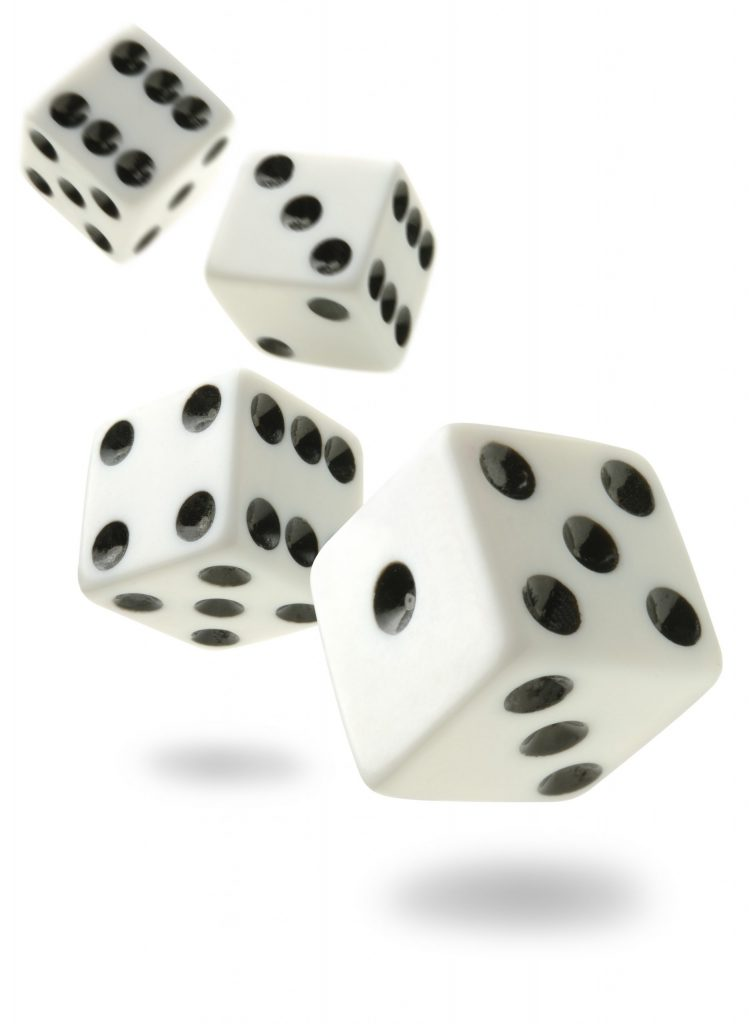
\includegraphics[width=0.25\linewidth]{images/rolling-four-dice} 

}

\caption{Rolling 4 dice in Game version A}\label{fig:unnamed-chunk-19}
\end{figure}

You've also learned that we can write some code to play this game once,
determining the winning status:

\begin{Shaded}
\begin{Highlighting}[]
\CommentTok{\# playing Game{-}A once}
\FunctionTok{set.seed}\NormalTok{(}\DecValTok{20}\NormalTok{)}
\NormalTok{die }\OtherTok{=} \DecValTok{1}\SpecialCharTok{:}\DecValTok{6}
\NormalTok{four\_rolls }\OtherTok{=} \FunctionTok{sample}\NormalTok{(die, }\AttributeTok{size =} \DecValTok{4}\NormalTok{, }\AttributeTok{replace =} \ConstantTok{TRUE}\NormalTok{)}
\NormalTok{win }\OtherTok{=} \FunctionTok{any}\NormalTok{(four\_rolls)}
\NormalTok{win}
\end{Highlighting}
\end{Shaded}

\begin{verbatim}
## [1] TRUE
\end{verbatim}

\hypertarget{playing-game-a-five-times}{%
\section{Playing Game-A Five Times}\label{playing-game-a-five-times}}

We are ready to write code and use it to play Game-A five times

\begin{Shaded}
\begin{Highlighting}[]
\FunctionTok{set.seed}\NormalTok{(}\DecValTok{133}\NormalTok{)}

\NormalTok{die }\OtherTok{=} \DecValTok{1}\SpecialCharTok{:}\DecValTok{6}

\NormalTok{game\_1 }\OtherTok{=} \FunctionTok{sample}\NormalTok{(die, }\AttributeTok{size =} \DecValTok{4}\NormalTok{, }\AttributeTok{replace =} \ConstantTok{TRUE}\NormalTok{)}
\NormalTok{game\_2 }\OtherTok{=} \FunctionTok{sample}\NormalTok{(die, }\AttributeTok{size =} \DecValTok{4}\NormalTok{, }\AttributeTok{replace =} \ConstantTok{TRUE}\NormalTok{)}
\NormalTok{game\_3 }\OtherTok{=} \FunctionTok{sample}\NormalTok{(die, }\AttributeTok{size =} \DecValTok{4}\NormalTok{, }\AttributeTok{replace =} \ConstantTok{TRUE}\NormalTok{)}
\NormalTok{game\_4 }\OtherTok{=} \FunctionTok{sample}\NormalTok{(die, }\AttributeTok{size =} \DecValTok{4}\NormalTok{, }\AttributeTok{replace =} \ConstantTok{TRUE}\NormalTok{)}
\NormalTok{game\_5 }\OtherTok{=} \FunctionTok{sample}\NormalTok{(die, }\AttributeTok{size =} \DecValTok{4}\NormalTok{, }\AttributeTok{replace =} \ConstantTok{TRUE}\NormalTok{)}

\CommentTok{\# win (or lose)?}
\NormalTok{wins }\OtherTok{=} \FunctionTok{c}\NormalTok{(}
  \StringTok{"game\_1"} \OtherTok{=} \FunctionTok{any}\NormalTok{(game\_1 }\SpecialCharTok{==} \DecValTok{6}\NormalTok{),}
  \StringTok{"game\_2"} \OtherTok{=} \FunctionTok{any}\NormalTok{(game\_2 }\SpecialCharTok{==} \DecValTok{6}\NormalTok{),}
  \StringTok{"game\_3"} \OtherTok{=} \FunctionTok{any}\NormalTok{(game\_3 }\SpecialCharTok{==} \DecValTok{6}\NormalTok{),}
  \StringTok{"game\_4"} \OtherTok{=} \FunctionTok{any}\NormalTok{(game\_4 }\SpecialCharTok{==} \DecValTok{6}\NormalTok{),}
  \StringTok{"game\_5"} \OtherTok{=} \FunctionTok{any}\NormalTok{(game\_5 }\SpecialCharTok{==} \DecValTok{6}\NormalTok{))}
  
\CommentTok{\# number of wins}
\NormalTok{total\_wins }\OtherTok{=} \FunctionTok{sum}\NormalTok{(wins)}
\NormalTok{total\_wins}
\end{Highlighting}
\end{Shaded}

\begin{verbatim}
## [1] 3
\end{verbatim}

\begin{Shaded}
\begin{Highlighting}[]
\CommentTok{\# proportion of wins}
\NormalTok{prop\_wins }\OtherTok{=} \FunctionTok{sum}\NormalTok{(wins) }\SpecialCharTok{/} \DecValTok{5}
\NormalTok{prop\_wins}
\end{Highlighting}
\end{Shaded}

\begin{verbatim}
## [1] 0.6
\end{verbatim}

As you can tell, the above code works, but there is a substantial amount of
unnecessary repetition. Imagine copying-pasting the \texttt{sample()} command
if we wanted to play Game-A 50 times, or 100 times, or 1000 times.

\hypertarget{using-a-for-loop}{%
\section{\texorpdfstring{Using a \texttt{for()} loop}{Using a for() loop}}\label{using-a-for-loop}}

The above code generates the five following games (each game with 4 rolls)

\begin{center}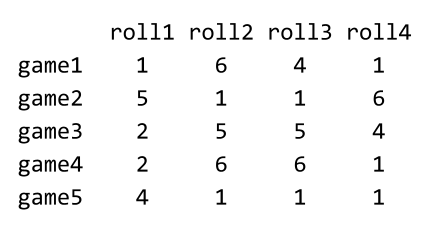
\includegraphics[width=0.4\linewidth]{images/demere-5-games} \end{center}

To avoid repeating the same commands multiple times, we can take advantage of
loops, for example with a \texttt{for()} loop.

Instead of using individual vectors \texttt{game\_1}, \texttt{game\_2}, etc, we are going to
use a matrix to store the rolls of all games. One option for this matrix is to
initialize it in a way that rows correspond to games, while columns correspond
to rolls:

\begin{figure}

{\centering 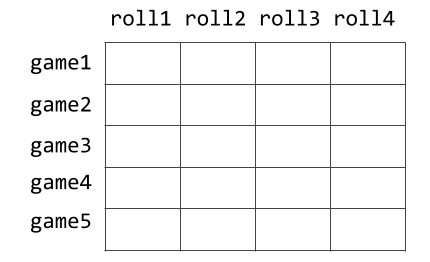
\includegraphics[width=0.4\linewidth]{images/demere-5-games-matrix} 

}

\caption{Structure of output matrix with 5 rows and 4 columns.}\label{fig:unnamed-chunk-23}
\end{figure}

The idea is to have an iterative process in which each iteration is associated
to a game. In other words, at each iteration we play a single game, and we
store the output of the rolls in the associated row of the matrix. Here's how.

\begin{Shaded}
\begin{Highlighting}[]
\FunctionTok{set.seed}\NormalTok{(}\DecValTok{133}\NormalTok{)}

\NormalTok{die }\OtherTok{=} \DecValTok{1}\SpecialCharTok{:}\DecValTok{6}
\NormalTok{number\_games }\OtherTok{=} \DecValTok{5}

\CommentTok{\# initialize output matrix (full of zeros)}
\NormalTok{games }\OtherTok{=} \FunctionTok{matrix}\NormalTok{(}\DecValTok{0}\NormalTok{, }\AttributeTok{nrow =}\NormalTok{ number\_games, }\AttributeTok{ncol =} \DecValTok{4}\NormalTok{)}

\CommentTok{\# each iteration corresponds to a single game}
\ControlFlowTok{for}\NormalTok{ (game }\ControlFlowTok{in} \DecValTok{1}\SpecialCharTok{:}\NormalTok{number\_games) \{}
\NormalTok{  games[game, ] }\OtherTok{=} \FunctionTok{sample}\NormalTok{(die, }\AttributeTok{size =} \DecValTok{4}\NormalTok{, }\AttributeTok{replace =} \ConstantTok{TRUE}\NormalTok{)}
\NormalTok{\}}

\FunctionTok{rownames}\NormalTok{(games) }\OtherTok{=} \FunctionTok{paste0}\NormalTok{(}\StringTok{"game"}\NormalTok{, }\DecValTok{1}\SpecialCharTok{:}\NormalTok{number\_games)}
\FunctionTok{colnames}\NormalTok{(games) }\OtherTok{=} \FunctionTok{paste0}\NormalTok{(}\StringTok{"roll"}\NormalTok{, }\DecValTok{1}\SpecialCharTok{:}\DecValTok{4}\NormalTok{)}
\NormalTok{games}
\end{Highlighting}
\end{Shaded}

\begin{verbatim}
##       roll1 roll2 roll3 roll4
## game1     1     6     4     1
## game2     5     1     1     6
## game3     2     5     5     4
## game4     2     6     6     1
## game5     4     1     1     1
\end{verbatim}

Observe the calls of \texttt{rownames()} and \texttt{colnames()} to assign names to both the
rows and the columns of the \texttt{games} matrix. In turn, the row and column names
are created with \texttt{paste0()} to generate the necessary character vectors.

\hypertarget{playing-game-a-10-times}{%
\section{Playing Game-A 10 times}\label{playing-game-a-10-times}}

Now that we have our \texttt{for()} loop in place, we can easily increase the number
of games. For instance, consider 10 games. Taking into account the preceding
code chunk, all we have to do is change the value of \texttt{number\_games}

\begin{Shaded}
\begin{Highlighting}[]
\FunctionTok{set.seed}\NormalTok{(}\DecValTok{133}\NormalTok{)}

\NormalTok{die }\OtherTok{=} \DecValTok{1}\SpecialCharTok{:}\DecValTok{6}
\NormalTok{number\_games }\OtherTok{=} \DecValTok{10}

\CommentTok{\# initialize output matrix}
\NormalTok{games }\OtherTok{=} \FunctionTok{matrix}\NormalTok{(}\DecValTok{0}\NormalTok{, }\AttributeTok{nrow =}\NormalTok{ number\_games, }\AttributeTok{ncol =} \DecValTok{4}\NormalTok{)}

\ControlFlowTok{for}\NormalTok{ (game }\ControlFlowTok{in} \DecValTok{1}\SpecialCharTok{:}\NormalTok{number\_games) \{}
\NormalTok{  games[game, ] }\OtherTok{=} \FunctionTok{sample}\NormalTok{(die, }\AttributeTok{size =} \DecValTok{4}\NormalTok{, }\AttributeTok{replace =} \ConstantTok{TRUE}\NormalTok{)}
\NormalTok{\}}

\FunctionTok{rownames}\NormalTok{(games) }\OtherTok{=} \FunctionTok{paste0}\NormalTok{(}\StringTok{"game"}\NormalTok{, }\DecValTok{1}\SpecialCharTok{:}\NormalTok{number\_games)}
\FunctionTok{colnames}\NormalTok{(games) }\OtherTok{=} \FunctionTok{paste0}\NormalTok{(}\StringTok{"roll"}\NormalTok{, }\DecValTok{1}\SpecialCharTok{:}\DecValTok{4}\NormalTok{)}
\NormalTok{games}
\end{Highlighting}
\end{Shaded}

\begin{verbatim}
##        roll1 roll2 roll3 roll4
## game1      1     6     4     1
## game2      5     1     1     6
## game3      2     5     5     4
## game4      2     6     6     1
## game5      4     1     1     1
## game6      4     3     4     2
## game7      6     3     1     3
## game8      4     2     1     1
## game9      1     6     2     1
## game10     5     1     6     5
\end{verbatim}

As you can tell, we now get a matrix \texttt{games} with 10 rows and 4
columns.

We still need to determine the status of each game: do we win? do we lose?

Conceptually, we could write another \texttt{for()} loop to determine the status of
each game: win or lose; something like this

\begin{Shaded}
\begin{Highlighting}[]
\CommentTok{\# initialize (logical) vector}
\NormalTok{wins }\OtherTok{=} \FunctionTok{logical}\NormalTok{(}\AttributeTok{length =}\NormalTok{ number\_games)}

\ControlFlowTok{for}\NormalTok{ (game }\ControlFlowTok{in} \DecValTok{1}\SpecialCharTok{:}\NormalTok{number\_games) \{}
\NormalTok{  wins[game] }\OtherTok{=} \FunctionTok{any}\NormalTok{(games[game, ] }\SpecialCharTok{==} \DecValTok{6}\NormalTok{)}
\NormalTok{\}}
\NormalTok{wins}
\end{Highlighting}
\end{Shaded}

\begin{verbatim}
##  [1]  TRUE  TRUE FALSE  TRUE FALSE FALSE  TRUE FALSE  TRUE  TRUE
\end{verbatim}

What are we doing in the preceding loop? Simply put, we are applying the
\texttt{any()} function to every row of matrix \texttt{games} to see if any of the row
elements are equal to six. This is illustrated in the following diagram:

\begin{figure}

{\centering 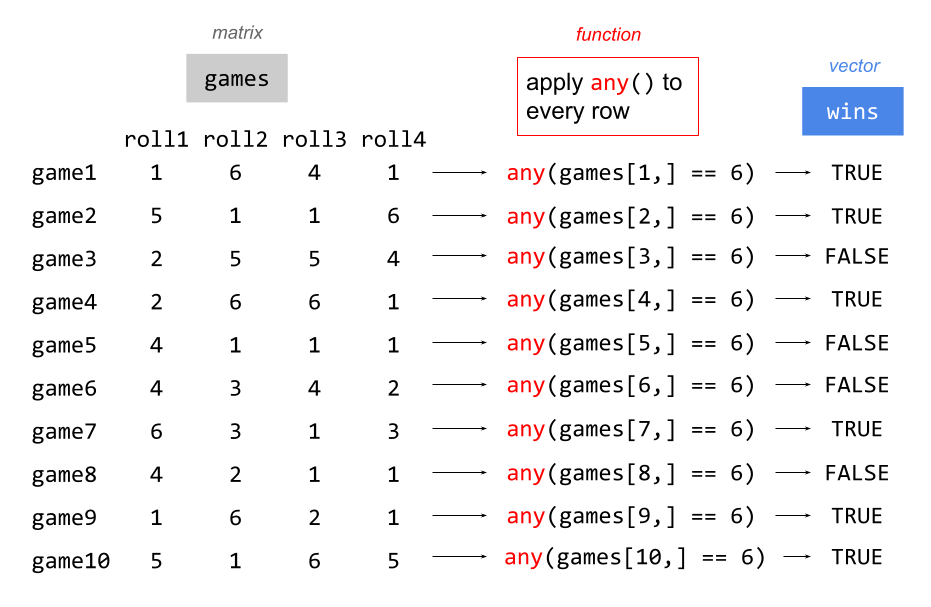
\includegraphics[width=0.9\linewidth]{images/demere-10-games-any} 

}

\caption{Diagram depicting the application of any() to all the rows of matrix games.}\label{fig:unnamed-chunk-27}
\end{figure}

While there is nothing conceptually wrong with the above \texttt{for()} loop, we can
advantage of other functions in R to help us write code in a more compact way.
Let's learn about this topic in the next chapter.

\hypertarget{vectorized-loops-with-apply}{%
\chapter{\texorpdfstring{Vectorized loops with \texttt{apply()}}{Vectorized loops with apply()}}\label{vectorized-loops-with-apply}}

We finish the last chapter writing code that simulates playing Game-A 10 times.
For recap purposes, the implemented code is displayed below:

\begin{Shaded}
\begin{Highlighting}[]
\FunctionTok{set.seed}\NormalTok{(}\DecValTok{133}\NormalTok{)}

\NormalTok{die }\OtherTok{=} \DecValTok{1}\SpecialCharTok{:}\DecValTok{6}
\NormalTok{number\_games }\OtherTok{=} \DecValTok{10}

\CommentTok{\# initialize output matrix}
\NormalTok{games }\OtherTok{=} \FunctionTok{matrix}\NormalTok{(}\DecValTok{0}\NormalTok{, }\AttributeTok{nrow =}\NormalTok{ number\_games, }\AttributeTok{ncol =} \DecValTok{4}\NormalTok{)}

\ControlFlowTok{for}\NormalTok{ (game }\ControlFlowTok{in} \DecValTok{1}\SpecialCharTok{:}\NormalTok{number\_games) \{}
\NormalTok{  games[game, ] }\OtherTok{=} \FunctionTok{sample}\NormalTok{(die, }\AttributeTok{size =} \DecValTok{4}\NormalTok{, }\AttributeTok{replace =} \ConstantTok{TRUE}\NormalTok{)}
\NormalTok{\}}

\FunctionTok{rownames}\NormalTok{(games) }\OtherTok{=} \FunctionTok{paste0}\NormalTok{(}\StringTok{"game"}\NormalTok{, }\DecValTok{1}\SpecialCharTok{:}\NormalTok{number\_games)}
\FunctionTok{colnames}\NormalTok{(games) }\OtherTok{=} \FunctionTok{paste0}\NormalTok{(}\StringTok{"roll"}\NormalTok{, }\DecValTok{1}\SpecialCharTok{:}\DecValTok{4}\NormalTok{)}
\NormalTok{games}
\end{Highlighting}
\end{Shaded}

The punchline of this piece of code has to do with the \texttt{for()} loop, storing
the outputs of each game in the rows of the \texttt{games} matrix.

Additionally, we also wrote a second \texttt{for()} loop to determine whether each
game---each row in \texttt{games}---had at least one six; this was done with the
\texttt{any()} function. This is illustrated in the following diagram:

\begin{figure}

{\centering 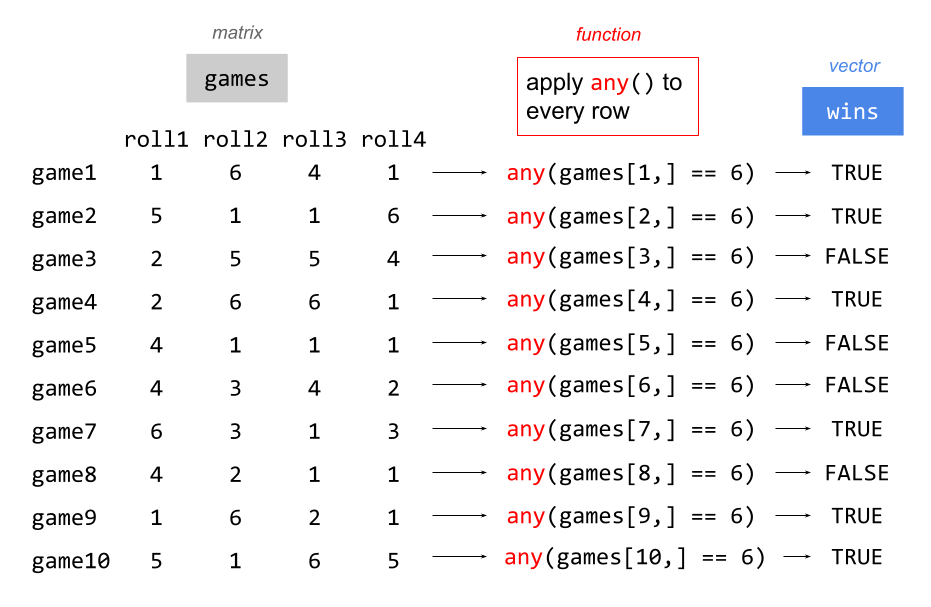
\includegraphics[width=0.9\linewidth]{images/demere-10-games-any} 

}

\caption{Diagram depicting the application of any() to all the rows of matrix games.}\label{fig:unnamed-chunk-29}
\end{figure}

\hypertarget{function-apply}{%
\section{\texorpdfstring{Function \texttt{apply()}}{Function apply()}}\label{function-apply}}

Instead of writing a loop to see which games are wins, and which games are
losses, we can take advantage of a very interesting function called \texttt{apply()},
which R users refer to as a \emph{vectorized loop} function.

As the name indicates, \texttt{apply()} lets you \textbf{apply} a function to the elements
of a matrix. The elements of a matrix can be:

\begin{itemize}
\item
  its rows: \texttt{MARGIN\ =\ 1}
\item
  its columns: \texttt{MARGIN\ =\ 2}
\item
  both (rows \& cols): \texttt{MARGIN\ =\ c(1,\ 2)}
\end{itemize}

For example, say you want to get the \texttt{sum()} of all the elements in each
row of \texttt{games}:

\begin{Shaded}
\begin{Highlighting}[]
\CommentTok{\# row sum}
\FunctionTok{apply}\NormalTok{(}\AttributeTok{X =}\NormalTok{ games, }\AttributeTok{MARGIN =} \DecValTok{1}\NormalTok{, }\AttributeTok{FUN =}\NormalTok{ sum)}
\end{Highlighting}
\end{Shaded}

\begin{verbatim}
##  game1  game2  game3  game4  game5  game6  game7  game8  game9 game10 
##     12     13     16     15      7     13     13      8     10     17
\end{verbatim}

We pass three inputs to \texttt{apply()}. The first ingredient is the input matrix,
the second ingredient specifies the \texttt{MARGIN} value, and the third ingredient
is the function to be applied.

Here's another example. Say you want to obtain the product of all the elements
in each column of \texttt{games}:

\begin{Shaded}
\begin{Highlighting}[]
\CommentTok{\# column product}
\FunctionTok{apply}\NormalTok{(}\AttributeTok{X =}\NormalTok{ games, }\AttributeTok{MARGIN =} \DecValTok{2}\NormalTok{, }\AttributeTok{FUN =}\NormalTok{ prod)}
\end{Highlighting}
\end{Shaded}

\begin{verbatim}
## roll1 roll2 roll3 roll4 
## 38400 19440  5760   720
\end{verbatim}

Or what if you want to get the minimum in each row of \texttt{games}:

\begin{Shaded}
\begin{Highlighting}[]
\CommentTok{\# row minimum}
\FunctionTok{apply}\NormalTok{(}\AttributeTok{X =}\NormalTok{ games, }\AttributeTok{MARGIN =} \DecValTok{1}\NormalTok{, }\AttributeTok{FUN =}\NormalTok{ min)}
\end{Highlighting}
\end{Shaded}

\begin{verbatim}
##  game1  game2  game3  game4  game5  game6  game7  game8  game9 game10 
##      1      1      2      1      1      2      1      1      1      1
\end{verbatim}

\hypertarget{anonymous-functions-and-apply}{%
\section{\texorpdfstring{Anonymous functions and \texttt{apply()}}{Anonymous functions and apply()}}\label{anonymous-functions-and-apply}}

Some times, there is no built-in function to do what we want. For instance,
say you want to obtain the \textbf{range} of each row, that is, the maximum minus
the minimum. R has a \texttt{range()} function but it does not return a single value,
it just gives you the min and the max of an input vector:

\begin{Shaded}
\begin{Highlighting}[]
\NormalTok{game\_1 }\OtherTok{=} \FunctionTok{c}\NormalTok{(}\DecValTok{1}\NormalTok{, }\DecValTok{6}\NormalTok{, }\DecValTok{4}\NormalTok{, }\DecValTok{1}\NormalTok{)}
\FunctionTok{range}\NormalTok{(game\_1)}
\end{Highlighting}
\end{Shaded}

\begin{verbatim}
## [1] 1 6
\end{verbatim}

If you want the range, you need to compute the \texttt{max()} minus the \texttt{min()}

\begin{Shaded}
\begin{Highlighting}[]
\NormalTok{game\_1 }\OtherTok{=} \FunctionTok{c}\NormalTok{(}\DecValTok{1}\NormalTok{, }\DecValTok{6}\NormalTok{, }\DecValTok{4}\NormalTok{, }\DecValTok{1}\NormalTok{)}
\NormalTok{range\_1 }\OtherTok{=} \FunctionTok{max}\NormalTok{(game\_1) }\SpecialCharTok{{-}} \FunctionTok{min}\NormalTok{(game\_1)}
\NormalTok{range\_1}
\end{Highlighting}
\end{Shaded}

\begin{verbatim}
## [1] 5
\end{verbatim}

Because R does not have a built-in function that returns the range, we need
to provide this function for the \texttt{FUN} argument of \texttt{apply()}. When the function
to be provided is fairly simple, we can create an \textbf{anonymous function}
inside \texttt{apply()}:

\begin{Shaded}
\begin{Highlighting}[]
\CommentTok{\# row ranges (with anonymous function)}
\FunctionTok{apply}\NormalTok{(}
  \AttributeTok{X =}\NormalTok{ games, }
  \AttributeTok{MARGIN =} \DecValTok{1}\NormalTok{, }
  \AttributeTok{FUN =} \ControlFlowTok{function}\NormalTok{(x) }\FunctionTok{max}\NormalTok{(x) }\SpecialCharTok{{-}} \FunctionTok{min}\NormalTok{(x))}
\end{Highlighting}
\end{Shaded}

\begin{verbatim}
##  game1  game2  game3  game4  game5  game6  game7  game8  game9 game10 
##      5      5      3      5      3      2      5      3      5      5
\end{verbatim}

The reason why the provided function to \texttt{FUN} is called an anonymous function
is because the created function has no name.

An alternative option is to first create a function outside \texttt{apply()}, and
then pass this function like any other function. This alternative is often
preferred when the body of the function to be passed to \texttt{apply()} involves
several lines of code.

\begin{Shaded}
\begin{Highlighting}[]
\CommentTok{\# auxiliary function to compute range}
\NormalTok{vector\_range }\OtherTok{=} \ControlFlowTok{function}\NormalTok{(x) \{}
  \FunctionTok{max}\NormalTok{(x) }\SpecialCharTok{{-}} \FunctionTok{min}\NormalTok{(x)}
\NormalTok{\}}

\CommentTok{\# row ranges}
\FunctionTok{apply}\NormalTok{(}
  \AttributeTok{X =}\NormalTok{ games, }
  \AttributeTok{MARGIN =} \DecValTok{1}\NormalTok{, }
\NormalTok{  vector\_range)}
\end{Highlighting}
\end{Shaded}

\begin{verbatim}
##  game1  game2  game3  game4  game5  game6  game7  game8  game9 game10 
##      5      5      3      5      3      2      5      3      5      5
\end{verbatim}

\hypertarget{number-of-wins-with-apply}{%
\subsection{\texorpdfstring{Number of wins with \texttt{apply()}}{Number of wins with apply()}}\label{number-of-wins-with-apply}}

Because there's no default function that computes if \texttt{any()} element of a
vector is equal to six, we need to create an \emph{anonymous} function for the
\texttt{FUN} argument:

\begin{Shaded}
\begin{Highlighting}[]
\NormalTok{wins }\OtherTok{=} \FunctionTok{apply}\NormalTok{(}
  \AttributeTok{X =}\NormalTok{ games, }
  \AttributeTok{MARGIN =} \DecValTok{1}\NormalTok{,}
  \AttributeTok{FUN =} \ControlFlowTok{function}\NormalTok{(x) }\FunctionTok{any}\NormalTok{(x }\SpecialCharTok{==} \DecValTok{6}\NormalTok{))}

\NormalTok{wins}
\end{Highlighting}
\end{Shaded}

\begin{verbatim}
##  game1  game2  game3  game4  game5  game6  game7  game8  game9 game10 
##   TRUE   TRUE  FALSE   TRUE  FALSE  FALSE   TRUE  FALSE   TRUE   TRUE
\end{verbatim}

We can now compute the proportion of wins:

\begin{Shaded}
\begin{Highlighting}[]
\NormalTok{prop\_wins }\OtherTok{=} \FunctionTok{sum}\NormalTok{(wins) }\SpecialCharTok{/}\NormalTok{ number\_games}
\NormalTok{prop\_wins}
\end{Highlighting}
\end{Shaded}

\begin{verbatim}
## [1] 0.6
\end{verbatim}

\hypertarget{playing-game-a-100-times}{%
\chapter{Playing Game-A 100 times}\label{playing-game-a-100-times}}

With all the coding elements that we have so far, it's time to play Game-A 100
times, and see what the proportion of wins turns out to be:

\begin{Shaded}
\begin{Highlighting}[]
\CommentTok{\# random seed (for reproducibility purposes)}
\FunctionTok{set.seed}\NormalTok{(}\DecValTok{753}\NormalTok{)}

\CommentTok{\# main inputs}
\NormalTok{die }\OtherTok{=} \DecValTok{1}\SpecialCharTok{:}\DecValTok{6}
\NormalTok{number\_games }\OtherTok{=} \DecValTok{100}

\CommentTok{\# initialize output matrix}
\NormalTok{games }\OtherTok{=} \FunctionTok{matrix}\NormalTok{(}\DecValTok{0}\NormalTok{, }\AttributeTok{nrow =}\NormalTok{ number\_games, }\AttributeTok{ncol =} \DecValTok{4}\NormalTok{)}

\CommentTok{\# playing Game{-}A several times}
\ControlFlowTok{for}\NormalTok{ (game }\ControlFlowTok{in} \DecValTok{1}\SpecialCharTok{:}\NormalTok{number\_games) \{}
\NormalTok{  games[game, ] }\OtherTok{=} \FunctionTok{sample}\NormalTok{(die, }\AttributeTok{size =} \DecValTok{4}\NormalTok{, }\AttributeTok{replace =} \ConstantTok{TRUE}\NormalTok{)}
\NormalTok{\}}

\FunctionTok{rownames}\NormalTok{(games) }\OtherTok{=} \FunctionTok{paste0}\NormalTok{(}\StringTok{"game"}\NormalTok{, }\DecValTok{1}\SpecialCharTok{:}\NormalTok{number\_games)}
\FunctionTok{colnames}\NormalTok{(games) }\OtherTok{=} \FunctionTok{paste0}\NormalTok{(}\StringTok{"roll"}\NormalTok{, }\DecValTok{1}\SpecialCharTok{:}\DecValTok{4}\NormalTok{)}

\CommentTok{\# determine each game\textquotesingle{}s win{-}or{-}lose output}
\NormalTok{wins }\OtherTok{=} \FunctionTok{apply}\NormalTok{(}
  \AttributeTok{X =}\NormalTok{ games, }
  \AttributeTok{MARGIN =} \DecValTok{1}\NormalTok{,}
  \AttributeTok{FUN =} \ControlFlowTok{function}\NormalTok{(x) }\FunctionTok{any}\NormalTok{(x }\SpecialCharTok{==} \DecValTok{6}\NormalTok{))}

\CommentTok{\# total proportion of wins}
\NormalTok{prop\_wins }\OtherTok{=} \FunctionTok{sum}\NormalTok{(wins) }\SpecialCharTok{/}\NormalTok{ number\_games}
\NormalTok{prop\_wins}
\end{Highlighting}
\end{Shaded}

\begin{verbatim}
## [1] 0.5
\end{verbatim}

\hypertarget{plotting-cumulative-gains}{%
\section{Plotting Cumulative Gains}\label{plotting-cumulative-gains}}

It would be nice to visualize the sequence of wins and losses. To make things
more interesting, let's assume that you are paid \$1 if you win a game, but also
that you pay \$1 if you lose a game. That is:

\begin{itemize}
\item
  gain \texttt{1} if you win a game
\item
  gain \texttt{-1} if you lose a game
\end{itemize}

\begin{Shaded}
\begin{Highlighting}[]
\CommentTok{\# vector of gains}
\NormalTok{gains }\OtherTok{=} \FunctionTok{rep}\NormalTok{(}\SpecialCharTok{{-}}\DecValTok{1}\NormalTok{, number\_games)  }\CommentTok{\# initialize with all {-}1 elements}
\NormalTok{gains[wins] }\OtherTok{=} \DecValTok{1}                \CommentTok{\# switch to +1 for every win}

\CommentTok{\# cumulative gains}
\NormalTok{cumulative\_gains }\OtherTok{=} \FunctionTok{cumsum}\NormalTok{(gains)}
\end{Highlighting}
\end{Shaded}

As you can tell, in this particular simulation of 100 games, the total
proportion of wins is 0.5, and the total gain is
0. You didn't gain any money, but you didn't
lose either.

Here's the graph using base \texttt{"graphics"} functions:

\begin{Shaded}
\begin{Highlighting}[]
\FunctionTok{plot}\NormalTok{(}\DecValTok{1}\SpecialCharTok{:}\NormalTok{number\_games, cumulative\_gains, }\AttributeTok{type =} \StringTok{\textquotesingle{}l\textquotesingle{}}\NormalTok{)}
\FunctionTok{abline}\NormalTok{(}\AttributeTok{h =} \DecValTok{0}\NormalTok{, }\AttributeTok{col =} \StringTok{"tomato"}\NormalTok{, }\AttributeTok{lty =} \DecValTok{2}\NormalTok{)}
\end{Highlighting}
\end{Shaded}

\hypertarget{running-various-simulations}{%
\chapter{Running Various Simulations}\label{running-various-simulations}}

A single series of 100 games may not be enough to fully
understand the probability behavior of Game-A. So let's see how to run various
simulations, all of them involving playing 100 games.

\textbf{Let's start small}. Meaning, let's begin with a handful of games, and a few
simulations. This will allow us to get a better idea of the objects and
commands we need to use in order to later generalize things with more games
and simulations.

Our starting point will involve 3 simulations, each one consisting of 5 games
as illustrated in the picture below.

\begin{center}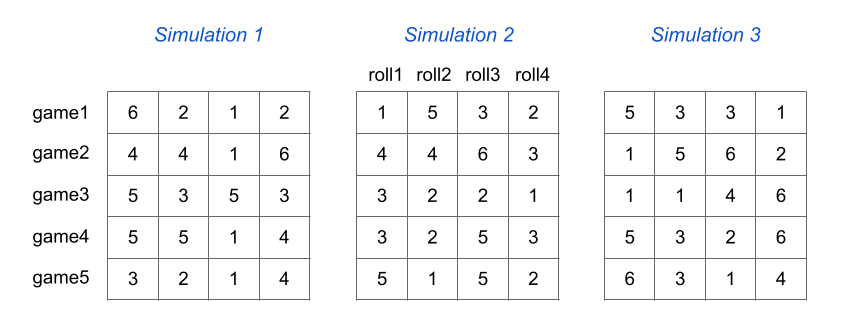
\includegraphics[width=0.8\linewidth]{images/demere-3-simulations} \end{center}

Here's some naive code to run these simulations. We are momentarily considering
this piece of code to get a high-level intuition of the things we might need
later to write more efficient commands.

\begin{Shaded}
\begin{Highlighting}[]
\CommentTok{\# {-}{-}{-}{-}{-}{-}{-}{-}{-}{-}{-}{-}{-}{-}{-}{-}{-}{-}{-}{-}{-}{-}{-}{-}{-}{-}{-}{-}{-}{-}{-}{-}{-}{-}{-}{-}{-}}
\CommentTok{\# three simulations, each of 5 games}
\CommentTok{\# {-}{-}{-}{-}{-}{-}{-}{-}{-}{-}{-}{-}{-}{-}{-}{-}{-}{-}{-}{-}{-}{-}{-}{-}{-}{-}{-}{-}{-}{-}{-}{-}{-}{-}{-}{-}{-}}

\FunctionTok{set.seed}\NormalTok{(}\DecValTok{753}\NormalTok{)}

\CommentTok{\# main inputs}
\NormalTok{die }\OtherTok{=} \DecValTok{1}\SpecialCharTok{:}\DecValTok{6}
\NormalTok{number\_games }\OtherTok{=} \DecValTok{5}

\CommentTok{\# simulation 1}
\NormalTok{games\_sim1 }\OtherTok{=} \FunctionTok{matrix}\NormalTok{(}\DecValTok{0}\NormalTok{, }\AttributeTok{nrow =}\NormalTok{ number\_games, }\AttributeTok{ncol =} \DecValTok{4}\NormalTok{)}
\ControlFlowTok{for}\NormalTok{ (game }\ControlFlowTok{in} \DecValTok{1}\SpecialCharTok{:}\NormalTok{number\_games) \{}
\NormalTok{  games\_sim1[game, ] }\OtherTok{=} \FunctionTok{sample}\NormalTok{(die, }\AttributeTok{size =} \DecValTok{4}\NormalTok{, }\AttributeTok{replace =} \ConstantTok{TRUE}\NormalTok{)}
\NormalTok{\}}
\NormalTok{wins\_sim1 }\OtherTok{=} \FunctionTok{apply}\NormalTok{(games\_sim1, }\DecValTok{1}\NormalTok{, }\ControlFlowTok{function}\NormalTok{(x) }\FunctionTok{any}\NormalTok{(x }\SpecialCharTok{==} \DecValTok{6}\NormalTok{))}
\NormalTok{prop\_wins\_sim1 }\OtherTok{=} \FunctionTok{sum}\NormalTok{(wins\_sim1) }\SpecialCharTok{/}\NormalTok{ number\_games}


\CommentTok{\# simulation 2}
\NormalTok{games\_sim2 }\OtherTok{=} \FunctionTok{matrix}\NormalTok{(}\DecValTok{0}\NormalTok{, }\AttributeTok{nrow =}\NormalTok{ number\_games, }\AttributeTok{ncol =} \DecValTok{4}\NormalTok{)}
\ControlFlowTok{for}\NormalTok{ (game }\ControlFlowTok{in} \DecValTok{1}\SpecialCharTok{:}\NormalTok{number\_games) \{}
\NormalTok{  games\_sim2[game, ] }\OtherTok{=} \FunctionTok{sample}\NormalTok{(die, }\AttributeTok{size =} \DecValTok{4}\NormalTok{, }\AttributeTok{replace =} \ConstantTok{TRUE}\NormalTok{)}
\NormalTok{\}}
\NormalTok{wins\_sim2 }\OtherTok{=} \FunctionTok{apply}\NormalTok{(games\_sim2, }\DecValTok{1}\NormalTok{, }\ControlFlowTok{function}\NormalTok{(x) }\FunctionTok{any}\NormalTok{(x }\SpecialCharTok{==} \DecValTok{6}\NormalTok{))}
\NormalTok{prop\_wins\_sim2 }\OtherTok{=} \FunctionTok{sum}\NormalTok{(wins\_sim2) }\SpecialCharTok{/}\NormalTok{ number\_games}


\CommentTok{\# simulation 3}
\NormalTok{games\_sim3 }\OtherTok{=} \FunctionTok{matrix}\NormalTok{(}\DecValTok{0}\NormalTok{, }\AttributeTok{nrow =}\NormalTok{ number\_games, }\AttributeTok{ncol =} \DecValTok{4}\NormalTok{)}
\ControlFlowTok{for}\NormalTok{ (game }\ControlFlowTok{in} \DecValTok{1}\SpecialCharTok{:}\NormalTok{number\_games) \{}
\NormalTok{  games\_sim3[game, ] }\OtherTok{=} \FunctionTok{sample}\NormalTok{(die, }\AttributeTok{size =} \DecValTok{4}\NormalTok{, }\AttributeTok{replace =} \ConstantTok{TRUE}\NormalTok{)}
\NormalTok{\}}
\NormalTok{wins\_sim3 }\OtherTok{=} \FunctionTok{apply}\NormalTok{(games\_sim3, }\DecValTok{1}\NormalTok{, }\ControlFlowTok{function}\NormalTok{(x) }\FunctionTok{any}\NormalTok{(x }\SpecialCharTok{==} \DecValTok{6}\NormalTok{))}
\NormalTok{prop\_wins\_sim3 }\OtherTok{=} \FunctionTok{sum}\NormalTok{(wins\_sim3) }\SpecialCharTok{/}\NormalTok{ number\_games}


\CommentTok{\# summary: proportion of wins}
\FunctionTok{c}\NormalTok{(}\StringTok{\textquotesingle{}sim1\textquotesingle{}} \OtherTok{=}\NormalTok{ prop\_wins\_sim1,}
  \StringTok{\textquotesingle{}sim2\textquotesingle{}} \OtherTok{=}\NormalTok{ prop\_wins\_sim2,}
  \StringTok{\textquotesingle{}sim3\textquotesingle{}} \OtherTok{=}\NormalTok{ prop\_wins\_sim3)}
\end{Highlighting}
\end{Shaded}

\begin{verbatim}
## sim1 sim2 sim3 
##  0.4  0.2  0.8
\end{verbatim}

This piece of code has a lot of unnecessary redundancy. But let's ignore this
fact for a second. In each simulation, we create a matrix \texttt{games\_sim} to store
the rolls of each game. Then we use \texttt{apply()} to determine which games are wins
(\texttt{wins\_sim}), and finally we calculate the proportion of wins (\texttt{prop\_wins\_sim}).

If you inspect the vectors \texttt{wins\_sim1}, \texttt{wins\_sim2}, and \texttt{wins\_sim3}, you'll
see that these are of \texttt{"logical"} data-type. \texttt{TRUE} means that a given game
is a win, whereas \texttt{FALSE} means lose.

Alternatively, instead of dealing with the logical vectors \texttt{wins\_sim}, we
can convert their values into numbers: \texttt{1} instead of \texttt{TRUE}, and \texttt{-1} instead
of \texttt{FALSE}. Why do we need this change from logical to numbers? Quick
answer, you don't really need it. But as we'll see, working with \texttt{1} and \texttt{-1}
is more convenient later down the road when we calculate expected gains.

The diagram below depicts this idea of storing the end result of each game
into \texttt{1} (win) or \texttt{-1} (lose), for every simulation:

\begin{center}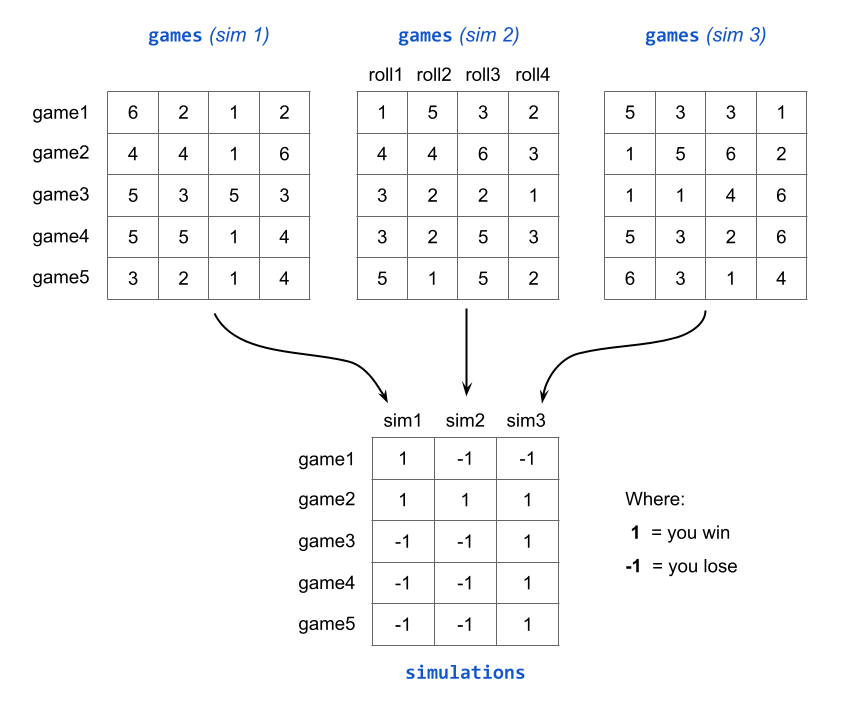
\includegraphics[width=0.8\linewidth]{images/demere-3-sims-loop} \end{center}

\hypertarget{embedded-for-loops}{%
\section{\texorpdfstring{Embedded \texttt{for()} loops}{Embedded for() loops}}\label{embedded-for-loops}}

Let's take the preceding naive code and try to make it more compact. We are
going to use embedded \texttt{for()} loops: one of them to take care of the simulations,
and the other one to take care of the games.

The idea is to iterate through each simulation: 1, 2, and 3. And then, in a
given simulation, we iterate through each game: 1, 2, 3, 4, and 5.

\begin{Shaded}
\begin{Highlighting}[]
\FunctionTok{set.seed}\NormalTok{(}\DecValTok{753}\NormalTok{)}

\CommentTok{\# main inputs}
\NormalTok{die }\OtherTok{=} \DecValTok{1}\SpecialCharTok{:}\DecValTok{6}
\NormalTok{number\_games }\OtherTok{=} \DecValTok{5}
\NormalTok{number\_sims }\OtherTok{=} \DecValTok{3}

\CommentTok{\# matrix to store simulation outputs}
\NormalTok{simulations }\OtherTok{=} \FunctionTok{matrix}\NormalTok{(}\DecValTok{0}\NormalTok{, }\AttributeTok{nrow =}\NormalTok{ number\_games, }\AttributeTok{ncol =}\NormalTok{ number\_sims)}

\CommentTok{\# 1st loop) iterate through each simulation}
\ControlFlowTok{for}\NormalTok{ (sim }\ControlFlowTok{in} \DecValTok{1}\SpecialCharTok{:}\NormalTok{number\_sims) \{}
\NormalTok{  games }\OtherTok{=} \FunctionTok{matrix}\NormalTok{(}\DecValTok{0}\NormalTok{, }\AttributeTok{nrow =}\NormalTok{ number\_games, }\AttributeTok{ncol =} \DecValTok{4}\NormalTok{)}
  
  \CommentTok{\# 2nd loop) iterate through each game}
  \ControlFlowTok{for}\NormalTok{ (game }\ControlFlowTok{in} \DecValTok{1}\SpecialCharTok{:}\NormalTok{number\_games) \{}
\NormalTok{    games[game, ] }\OtherTok{=} \FunctionTok{sample}\NormalTok{(die, }\AttributeTok{size =} \DecValTok{4}\NormalTok{, }\AttributeTok{replace =} \ConstantTok{TRUE}\NormalTok{)}
\NormalTok{  \}}
\NormalTok{  any\_sixes }\OtherTok{=} \FunctionTok{apply}\NormalTok{(games, }\DecValTok{1}\NormalTok{, }\ControlFlowTok{function}\NormalTok{(x) }\FunctionTok{any}\NormalTok{(x }\SpecialCharTok{==} \DecValTok{6}\NormalTok{))}
\NormalTok{  simulations[ ,sim] }\OtherTok{=} \FunctionTok{ifelse}\NormalTok{(any\_sixes, }\DecValTok{1}\NormalTok{, }\SpecialCharTok{{-}}\DecValTok{1}\NormalTok{)}
\NormalTok{\}}

\FunctionTok{rownames}\NormalTok{(simulations) }\OtherTok{=} \FunctionTok{paste0}\NormalTok{(}\StringTok{"game"}\NormalTok{, }\DecValTok{1}\SpecialCharTok{:}\NormalTok{number\_games)}
\FunctionTok{colnames}\NormalTok{(simulations) }\OtherTok{=} \FunctionTok{paste0}\NormalTok{(}\StringTok{"sim"}\NormalTok{, }\DecValTok{1}\SpecialCharTok{:}\NormalTok{number\_sims)}
\NormalTok{simulations}
\end{Highlighting}
\end{Shaded}

\begin{verbatim}
##       sim1 sim2 sim3
## game1    1   -1   -1
## game2    1    1    1
## game3   -1   -1    1
## game4   -1   -1    1
## game5   -1   -1    1
\end{verbatim}

What's going on with this code? Before starting the iterations, we create a
matrix \texttt{simulations} which will store the numeric values of all games, and
all simulations. The rows of this matrix are associated to the games, while
the columns are associated to the simulations. At the end of the iterative
process, this matrix will be populated with \texttt{1} (win game) and \texttt{-1} (lose game).

The first \texttt{for()} loop iterates through the simulations. At the beginning of
each simulation, an auxiliary \texttt{games} matrix is initialized, which then gets
populated in the embedded \texttt{for()} loop. This second \texttt{for()} loop iterates
through the games, obtaining the rolls of the five games.
After the games are completed, we use \texttt{apply()} to determine which games are
wins (i.e.~have at least one 6), and then we convert the \texttt{TRUE}'s and \texttt{FALSE}'s
into \texttt{1} and \texttt{-1}, respectively, by using \texttt{ifelse()}. This numeric vector is
stored in the corresponding column of the \texttt{simulations} matrix.

Having obtained the matrix \texttt{simulations}, we then proceed to count the number
of wins \texttt{total\_wins} (see code below). Notice the use of \texttt{apply()} to count the
number of wins for each column of \texttt{simulations}. The last step involves
computing the proportion of wins \texttt{prop\_wins}:

\begin{Shaded}
\begin{Highlighting}[]
\NormalTok{total\_wins }\OtherTok{=} \FunctionTok{apply}\NormalTok{(simulations, }\DecValTok{2}\NormalTok{, }\ControlFlowTok{function}\NormalTok{(x) }\FunctionTok{sum}\NormalTok{(x}\SpecialCharTok{==}\DecValTok{1}\NormalTok{))}
\NormalTok{prop\_wins }\OtherTok{=}\NormalTok{ total\_wins }\SpecialCharTok{/}\NormalTok{ number\_games}
\NormalTok{prop\_wins}
\end{Highlighting}
\end{Shaded}

\begin{verbatim}
## sim1 sim2 sim3 
##  0.4  0.2  0.8
\end{verbatim}

\hypertarget{running-even-more-simulations}{%
\chapter{Running Even More Simulations}\label{running-even-more-simulations}}

In the previous section we discussed one possible strategy to run three
simulations, each one consisting of five games. From the programming point of
view, the core of this strategy is the utilization of embedded \texttt{for()} loops.

Now, three simulations and five games is obviously not enough. To get a better
feeling of the probability of winning Game-A---approximated by the proportion
of wins---we need to take things to the next level: with more simulations, and
many more games.

\begin{center}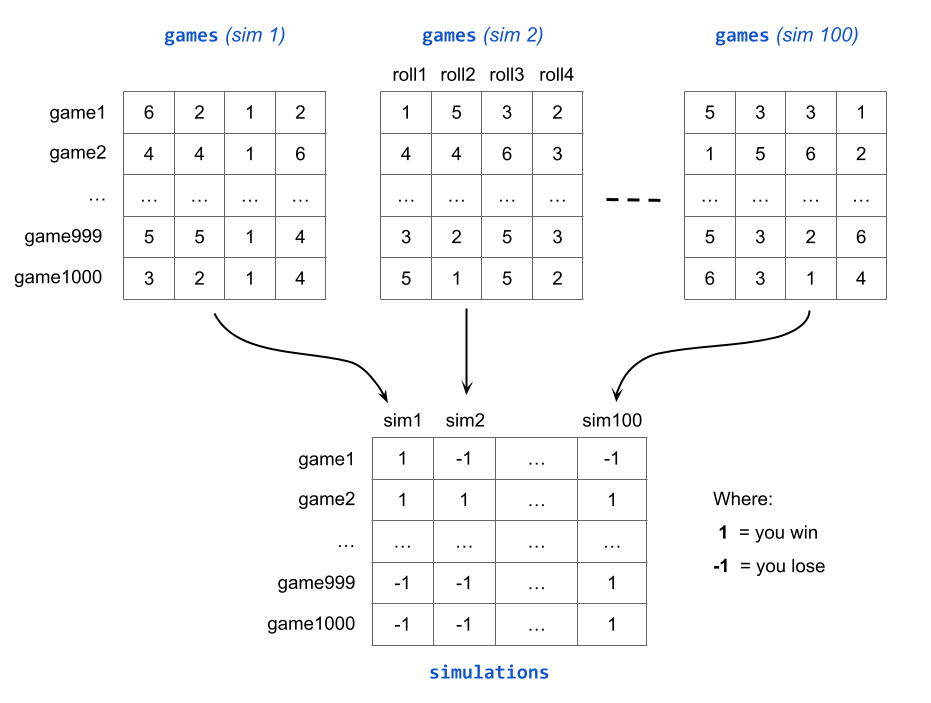
\includegraphics[width=0.9\linewidth]{images/demere-100-sims-loop} \end{center}

The following code uses 1000 games and 100 simulations. This allows us to
play Game-A for a total of \(1,000 \times 100 = 100,000\) times. With this many
games, we can safely calculate the average proportion of wins, and use this
value to estimate the probability of winning Game-A:

\begin{Shaded}
\begin{Highlighting}[]
\FunctionTok{set.seed}\NormalTok{(}\DecValTok{753}\NormalTok{)}

\CommentTok{\# main inputs}
\NormalTok{die }\OtherTok{=} \DecValTok{1}\SpecialCharTok{:}\DecValTok{6}
\NormalTok{number\_games }\OtherTok{=} \DecValTok{1000}
\NormalTok{number\_sims }\OtherTok{=} \DecValTok{100}

\CommentTok{\# matrix to store simulation outputs}
\NormalTok{simulations }\OtherTok{=} \FunctionTok{matrix}\NormalTok{(}\DecValTok{0}\NormalTok{, }\AttributeTok{nrow =}\NormalTok{ number\_games, }\AttributeTok{ncol =}\NormalTok{ number\_sims)}

\ControlFlowTok{for}\NormalTok{ (sim }\ControlFlowTok{in} \DecValTok{1}\SpecialCharTok{:}\NormalTok{number\_sims) \{}
\NormalTok{  games }\OtherTok{=} \FunctionTok{matrix}\NormalTok{(}\DecValTok{0}\NormalTok{, }\AttributeTok{nrow =}\NormalTok{ number\_games, }\AttributeTok{ncol =} \DecValTok{4}\NormalTok{)}
  \ControlFlowTok{for}\NormalTok{ (game }\ControlFlowTok{in} \DecValTok{1}\SpecialCharTok{:}\NormalTok{number\_games) \{}
\NormalTok{    games[game, ] }\OtherTok{=} \FunctionTok{sample}\NormalTok{(die, }\AttributeTok{size =} \DecValTok{4}\NormalTok{, }\AttributeTok{replace =} \ConstantTok{TRUE}\NormalTok{)}
\NormalTok{  \}}
\NormalTok{  any\_sixes }\OtherTok{=} \FunctionTok{apply}\NormalTok{(games, }\DecValTok{1}\NormalTok{, }\ControlFlowTok{function}\NormalTok{(x) }\FunctionTok{any}\NormalTok{(x }\SpecialCharTok{==} \DecValTok{6}\NormalTok{))}
\NormalTok{  simulations[ ,sim] }\OtherTok{=} \FunctionTok{ifelse}\NormalTok{(any\_sixes, }\DecValTok{1}\NormalTok{, }\SpecialCharTok{{-}}\DecValTok{1}\NormalTok{)}
\NormalTok{\}}

\FunctionTok{rownames}\NormalTok{(simulations) }\OtherTok{=} \FunctionTok{paste0}\NormalTok{(}\StringTok{"game"}\NormalTok{, }\DecValTok{1}\SpecialCharTok{:}\NormalTok{number\_games)}
\FunctionTok{colnames}\NormalTok{(simulations) }\OtherTok{=} \FunctionTok{paste0}\NormalTok{(}\StringTok{"sim"}\NormalTok{, }\DecValTok{1}\SpecialCharTok{:}\NormalTok{number\_sims)}

\NormalTok{total\_wins }\OtherTok{=} \FunctionTok{apply}\NormalTok{(simulations, }\DecValTok{2}\NormalTok{, }\ControlFlowTok{function}\NormalTok{(x) }\FunctionTok{sum}\NormalTok{(x}\SpecialCharTok{==}\DecValTok{1}\NormalTok{))}
\NormalTok{prop\_wins }\OtherTok{=}\NormalTok{ total\_wins }\SpecialCharTok{/}\NormalTok{ number\_games}

\CommentTok{\# mean win{-}proportion}
\FunctionTok{mean}\NormalTok{(prop\_wins)}
\end{Highlighting}
\end{Shaded}

\begin{verbatim}
## [1] 0.51674
\end{verbatim}

As you can tell, the average proportion of wins turns out to be 0.51674 which is pretty close to the theoretical probability of winning Game-A

\begin{align*}
Prob(\text{at least one six in 4 rolls}) &= 1 - Prob(\text{no six in 4 rolls}) \\
&= 1 - \left( \frac{5}{6} \right)^4 \\
&= 0.517747
\end{align*}

Of course, if you change the random seed and rerun this simulation, you will
very likely obtain a slightly different proportion of wins. But still close
enough to the actual theoretical probability of winning Game-A.

  \bibliography{book.bib}

\end{document}
